%   MSc Business Analytics Dissertation
%
%   Title:     Aaa Bbbbbbb Cccccccccc
%   Author(s): Xxxxxx Xxxxxxxxx and Yyy Yyyyyyyyy
%
%   Chapter 6: Discussion
%
%   Change Control:
%   When     Who   Ver  What
%   -------  ----  ---  --------------------------------------------------------------
%   11Feb11  AB    0.1  Begun 
%

\chapter{Discussion}\label{C.Discussion}

\section{Introduction}\label{S.Discussion.intro}

This chapter presents the detailed discussion and analysis of patterns and trends discovered during this research work. Keeping the interest of every stakeholder from bank officer to auditors, an attempt has been build simplicity in the business dashboard so that end user can use it efficiently to drive the business decision. When it was discovered that original data is not appropriate from the predictive modelling perspective, the modified data has been used throughout this research work. All analysis has been presented considering modified data set.

\section{Patterns \&  Analysis}

\begin{center}
\begin{figure}[!htb]
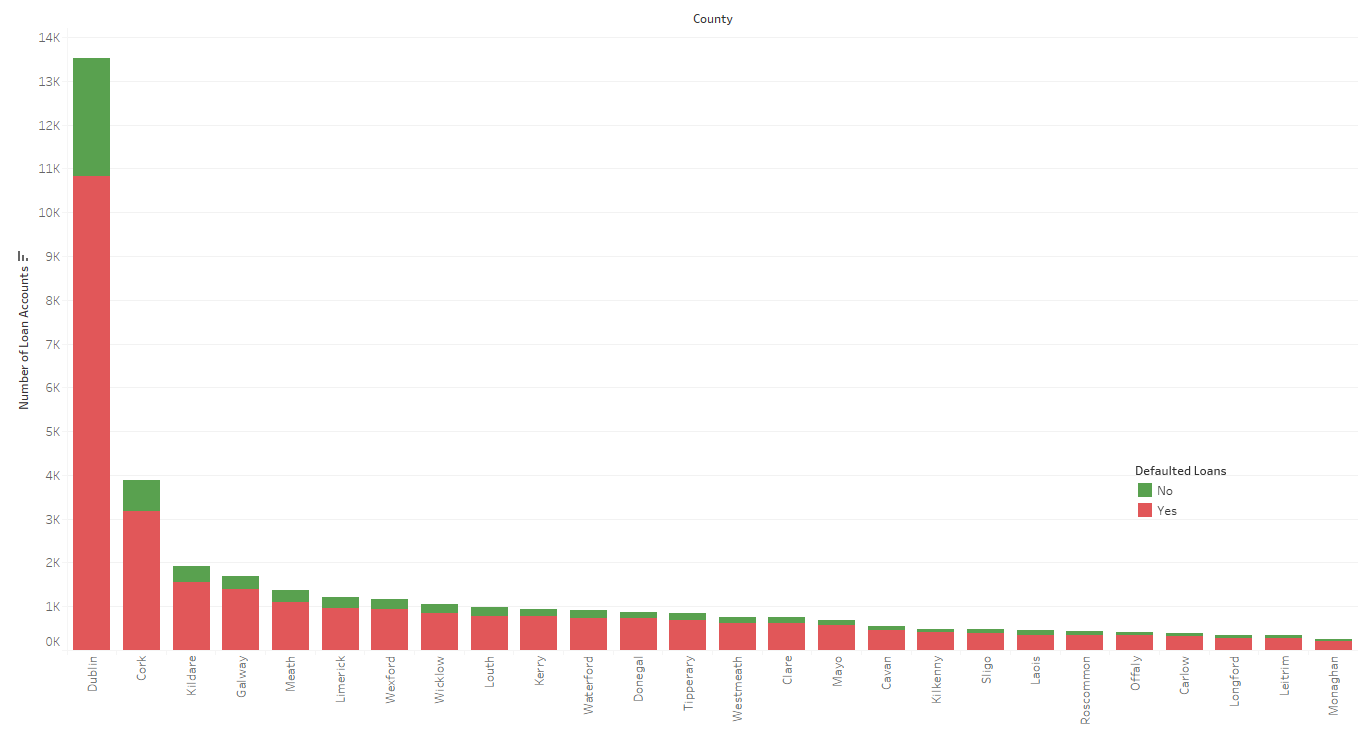
\includegraphics[width=\textwidth]{countynumber.png}
\centering
\caption{Number of account county wise}{\textbf{Source:} Tableau Pro}
\label{fig:tableaucounty}
\end{figure}
\end{center}

A total number of accounts in the modified data set was 36000, and most numbers of default and loan account were from County Dublin and Cork as seen in fig. \ref{fig:tableaucounty}.

\section{Success}\label{S.succes}

To measure the performance of this work, a working business dashboard has been given to stakeholder to use it and provide their feedback. Based on their feedback and suggestions dashboard features has been implemented accordingly. The user was given two dashboard design and asked to recommend best one with possible changes and suggestions to further improve usability.

\section{Integration with real data}

Credit scoring is a senstive and important component of any bank and financial institutions. The outcome of this work presents a predictive model that connects with a business dashboard. One can integrate the day to day financial data from a bank with this dashboard. This work can be improvised with the help of real banking data so that predictive model can be trained efficiently.

\begin{center}
\begin{figure}[!htb]
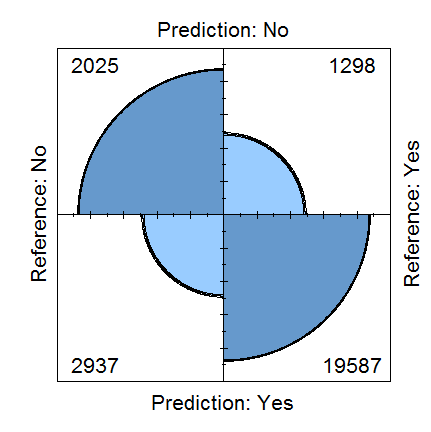
\includegraphics[width=\textwidth]{DTcm.png}
\centering
\caption{Confusion Matrix of Test Data}{\textbf{Source:} R Studio}
\label{fig:DTcm}
\end{figure}
\end{center}

By using open source library of R Shiny, a dynamic dashboard has been build which allow user to view property based on clustring. Also user can view street level statstical metrics.

\begin{center}
\begin{figure}[!htb]
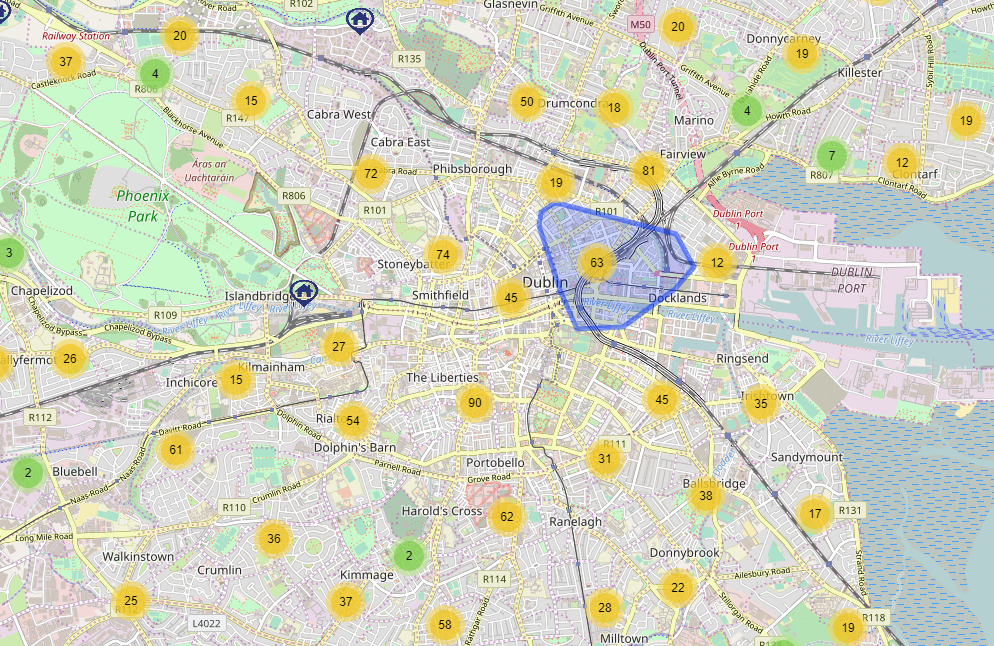
\includegraphics[width=\textwidth]{rmap.png}
\centering
\caption{Confusion Matrix of Test Data}{\textbf{Source:} R Studio}
\label{fig:rmap}
\end{figure}
\end{center}


